\section{Summary}
\label{sec:summary}

The prompt and non-prompt \jpsi and \psip \lth polarization parameters have been measured, 
in the helicity frame, 
using a sample of pp collisions at $\sqrt{s} = 13$\TeV collected in 2017 and 2018,
corresponding to an integrated luminosity of 103.3~fb$^{-1}$.
The results cover a very broad \pt range, extending up to \pt values around 100\GeV.

Figure~\ref{fig:Run2_vs_2011_jpsi_psip} compares the prompt \jpsi and \psip \lth measurements
obtained in this analysis,
with the results previously published by CMS, 
corresponding to pp collisions at $\sqrt{s} = 7$\TeV collected in 2011~\cite{bib:BPH-13-003}
(and already shown in Fig.~\ref{fig:BPH13003}).
%
Figure~\ref{fig:Run2_vs_2011_jpsi} shows only the \jpsi measurements,
for improved visibility. 

\begin{figure}[hb]
\centering
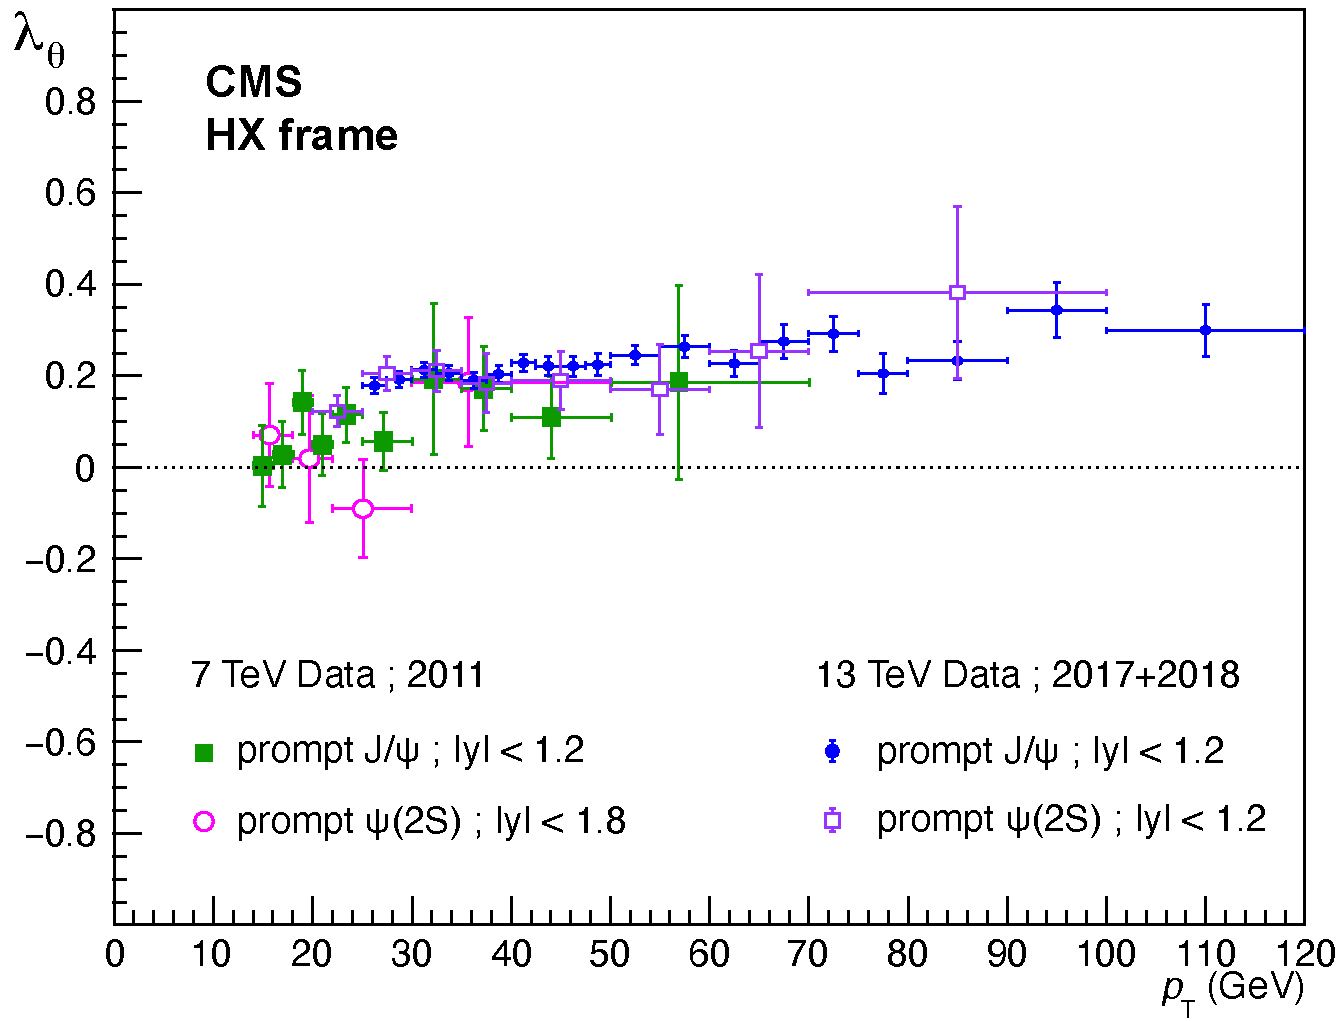
\includegraphics[width=0.6\textwidth]{Figures/chapter8/lth_HX-Run2-vs-2011-jpsi-psip.pdf}
\caption{\lth parameter measured, as a function of \pt, 
for prompt \jpsi and \psip mesons produced in pp collisions at $\sqrt{s} = 13$\TeV (this analysis)
and at $\sqrt{s} = 7$\TeV (BPH-13-003 analysis~\cite{bib:BPH-13-003}).
The vertical bars represent the statistical and systematic uncertainties 
summed in quadrature.}
\label{fig:Run2_vs_2011_jpsi_psip}
%\end{figure}
\vglue4mm
%\begin{figure}[h]
\centering
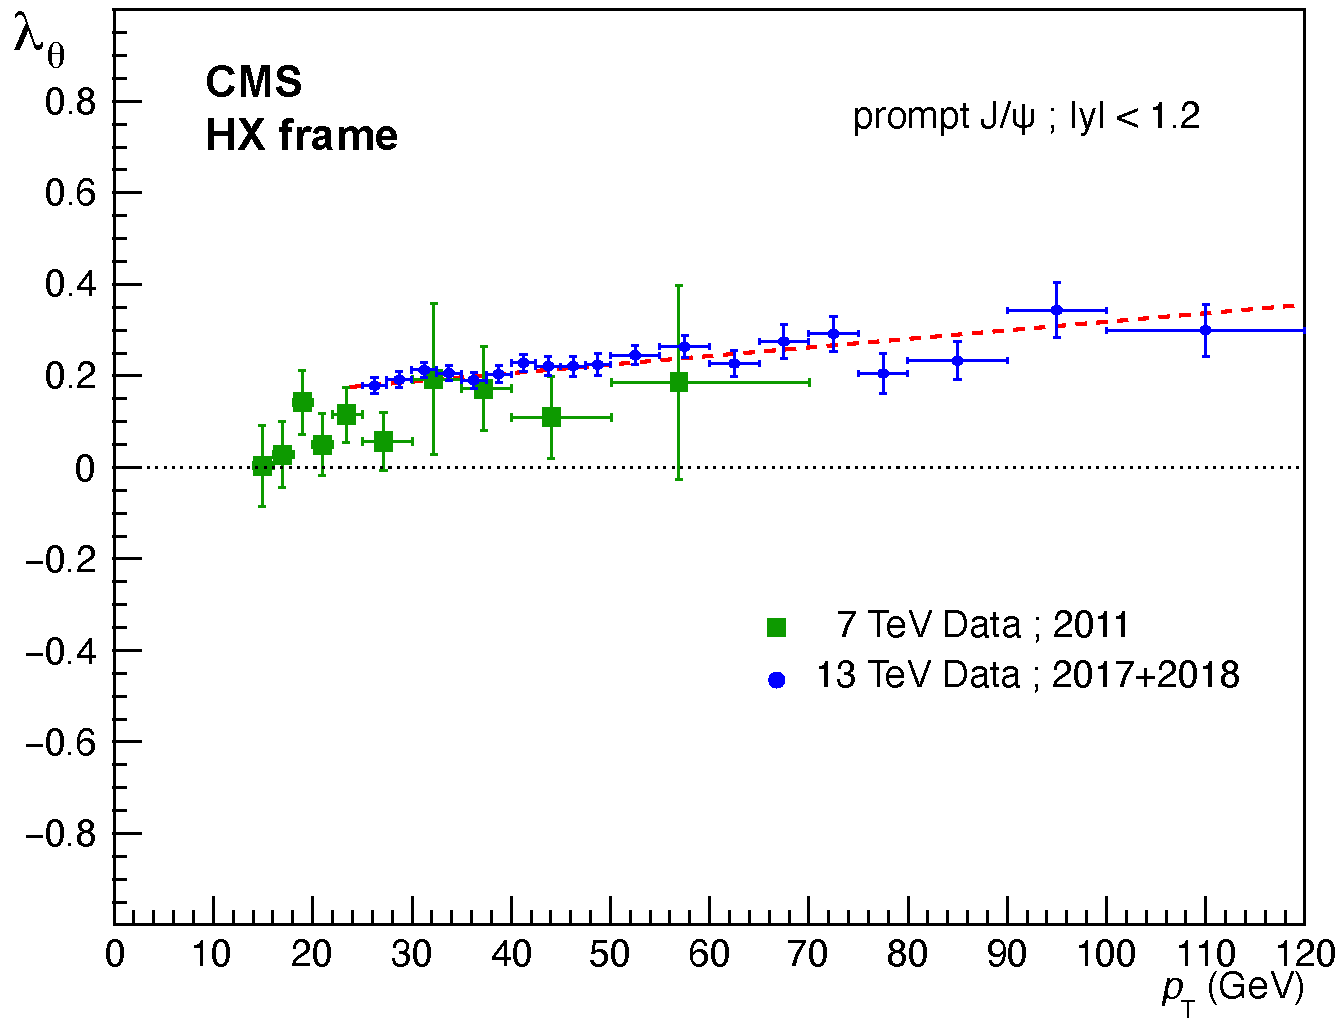
\includegraphics[width=0.6\textwidth]{Figures/chapter8/lth_HX-Run2-vs-2011-jpsi.pdf}
\caption{Same as the previous figure but without the \psip points,
to provide a better picture of the (more precise) \jpsi measurements.}
\label{fig:Run2_vs_2011_jpsi}
\end{figure}

\vfill\newpage

It is interesting to note that the 7\TeV measurements, albeit with large uncertainties, 
show \lth values that are closer to zero, in the 10--20\GeV \pt range,
than those we have measured in this analysis, at higher \pt,
for both the \jpsi and \psip results.
As indicated by the dashed red line in Fig.~\ref{fig:Run2_vs_2011_jpsi},
the values of \lth show a steady increase as \pt increases.

We see no evidence of strong transverse polarizations, 
even at \pt values around 30 times the \jpsi mass.
In the NRQCD language, we do not see evidence that, at very high \pt,
the transversely polarized ${}^3S_1^{[8]}$ octet term becomes dominant 
with respect to the unpolarized ${}^1S_0^{[8]}$ octet.

These results provide important constraints to be included 
in global analyses of quarkonium production.

